\documentclass[12pt,a4paper]{article}
\usepackage[UTF8]{ctex}
\usepackage{amsmath,amssymb}
\usepackage{xcolor}
\usepackage{hyperref}
\usepackage{geometry}
\usepackage{graphicx}
\geometry{margin=2.5cm}

\title{Elliptic Curve Cryptography / 椭圆曲线密码学}
\author{QuoNic}
\date{}

\begin{document}
\maketitle

\begin{center}
\textbf{Algorithms / 算法} | 难度：高级 | 预计时间：25 分钟
\end{center}

\tableofcontents
\newpage

\section{为什么需要？}

椭圆曲线密码学是基于椭圆曲线离散对数问题的密码系统。

\subsection{经典局限}
\begin{itemize}
  \item 经典算法需要指数时间求解 ECDLP
  \item 对于大参数，经典方法效率低
\end{itemize}

\subsection{量子优势}
\begin{itemize}
  \item 量子算法可以在多项式时间内求解 ECDLP
  \item 提供指数加速
  \item 是后量子密码学的基础
\end{itemize}

\subsection{实际应用}
\begin{itemize}
  \item 密码学
  \item 区块链
  \item 数字签名
\end{itemize}

\section{快速上手}

\begin{verbatim}
from quonic.algorithms import elliptic_curve

# 椭圆曲线离散对数
result = elliptic_curve(P=(3,6), Q=(7,8), a=2, p=97)
print(f'k = {result.k}')
\end{verbatim}

\textbf{预期输出}：
\begin{verbatim}
k = 3
\end{verbatim}

\section{原理详解}

\subsection{电路图}

\begin{center}
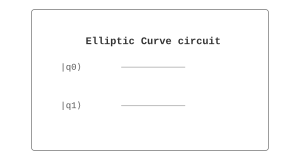
\includegraphics[width=0.6\textwidth]{../../images/elliptic_curve_circuit.svg}
\end{center}

\subsection{数学推导}

椭圆曲线：
\begin{equation}
y^2 = x^3 + ax + b \pmod{p}
\end{equation}

\textbf{离散对数}：
\begin{equation}
Q = kP
\end{equation}

其中 $P$ 是基点，$Q$ 是公钥，$k$ 是私钥。

\subsection{几何解释}

椭圆曲线上的点构成一个群。点加法和标量乘法是群运算。离散对数问题是从 $Q = kP$ 恢复 $k$。

\section{代码详解}

\begin{verbatim}
from quonic.algorithms import elliptic_curve

# elliptic_curve(P, Q, a, p)
# P: 基点
# Q: 公钥
# a: 曲线参数
# p: 素数模
result = elliptic_curve(P=(3,6), Q=(7,8), a=2, p=97)

# result.k: 私钥
# result.curve: 椭圆曲线
print(f'k = {result.k}')
\end{verbatim}

\section{进阶用法}

\subsection{场景 1：不同曲线}

\begin{verbatim}
from quonic.algorithms import elliptic_curve

# 不同椭圆曲线
result1 = elliptic_curve(P=(3,6), Q=(7,8), a=2, p=97)
result2 = elliptic_curve(P=(2,3), Q=(5,7), a=3, p=101)
print(f'Curve 1: k={result1.k}')
print(f'Curve 2: k={result2.k}')
\end{verbatim}

\section{适用场景}

\subsection{密码学}

椭圆曲线密码学是现代密码学的基础。比特币、以太坊等使用 ECDSA 签名验证交易。量子计算机可以从公钥恢复私钥，威胁椭圆曲线密码学的安全性。

\subsection{区块链}

椭圆曲线密码学是区块链安全的基础。量子计算机可以伪造数字签名，需要迁移到后量子密码学。

\section{常见问题}

\subsection{椭圆曲线密码学和 RSA 有什么区别？}

椭圆曲线密码学基于椭圆曲线离散对数问题，RSA 基于大整数分解问题。椭圆曲线密码学使用更短的密钥，效率更高。

\subsection{量子计算机能破解椭圆曲线密码学吗？}

是的，量子计算机可以在多项式时间内求解椭圆曲线离散对数问题。

\section{学习路径}

\subsection{前置知识}
\begin{itemize}
  \item 椭圆曲线
  \item 离散对数问题
  \item Shor 算法
\end{itemize}

\subsection{继续学习}
\begin{itemize}
  \item 后量子密码学
  \item 量子密钥分发
  \item 量子区块链
\end{itemize}

\section{完整示例代码}

\subsection{示例 1：基本椭圆曲线离散对数}

\begin{verbatim}
from quonic.algorithms import elliptic_curve

result = elliptic_curve(P=(3,6), Q=(7,8), a=2, p=97)
print(f'k = {result.k}')
\end{verbatim}

\section{下载}

\begin{itemize}
  \item [elliptic\_curve.py](https://github.com/ChrisLee0721/QuoNic/blob/main/examples/elliptic_curve/elliptic_curve.py)
\end{itemize}

\end{document}
